% !TEX root =  ../main_manuscript.tex 
\subsection{Statistical Methods}
For our aim to create risk of reclassification based personalized biopsy schedules, we required a risk prediction model. Available data was each patient's age at the start of AS, PSA measurements over follow-up, the timing of repeat biopsies and corresponding Gleason grades, and the time of reclassification (Figure~\ref{fig:delay_explanation}). Analysis of this data required modeling the correlation between the PSA measurements of the same patient, the correlation between the Gleason grade and the PSA profile, and to account for PSA measurements missing after a patient experienced reclassification. To this end, a commonly used model is the joint model for time-to-event and longitudinal data \citep{tomer2019,coley2017prediction,rizopoulos2012joint}.

%\begin{figure}[!htb]
%\centerline{\includegraphics[width=\columnwidth]{images/jm_blockdiag.pdf}}
%\caption{\textbf{Diagram of the joint model}: Patient-specific random effects (ellipse in center) are shared between sub-models for all outcomes pertaining to prostate cancer progression. The random effects model the correlation between the outcomes. In the linear mixed effects sub-model for $\log_2\{\mbox{PSA + 1}\}$ transformed PSA outcome (bottom rectangle), random effects are used as covariates. In the relative-risk sub-model (similar to Cox model) for time of Gleason~$\geq$~7 (GS7), random effects are utilized indirectly, by including fitted $\log_2\{\mbox{PSA + 1}\}$ value and velocities as covariates. Age of patient at baseline is included in both sub-models. Parameters of both sub-models are estimated jointly.}
%\label{fig:jm_blockdiag}
%\end{figure}

The joint model we utilized consisted of two sub-models. First, a linear mixed model \citep{laird1982random} for the longitudinally measured PSA (log-transformed). Second, a relative-risk model (similar to Cox model) for modeling the risk of reclassification using the observed times of reclassification. In the sub-model for PSA, we modeled PSA profiles non-linearly (Panel~A, Figure~\ref{fig:jmExplanationPlot_113}). From the fitted PSA profiles, we extracted the instantaneous PSA velocity for each patient. This instantaneous PSA velocity varies as the PSA profile varies over time (Panel~B, Figure~\ref{fig:jmExplanationPlot_113}). Thus it is more precise than the currently used PSA velocity/doubling-time \citep{vickers2009psavelocity}. We connected the two sub-models by using the fitted PSA profile and instantaneous PSA velocity as predictors for risk of reclassification in the relative-risk sub-model (Panel~C, Figure~\ref{fig:jmExplanationPlot_113}). Patient age was included as a predictor in both sub-models. The parameters of the two sub-models were estimated jointly using the R package \textbf{JMbayes} \citep{rizopoulosJMbayes}. This package utilizes the Bayesian methodology to estimate model parameters (Appendix~A). 

\begin{figure}
\centerline{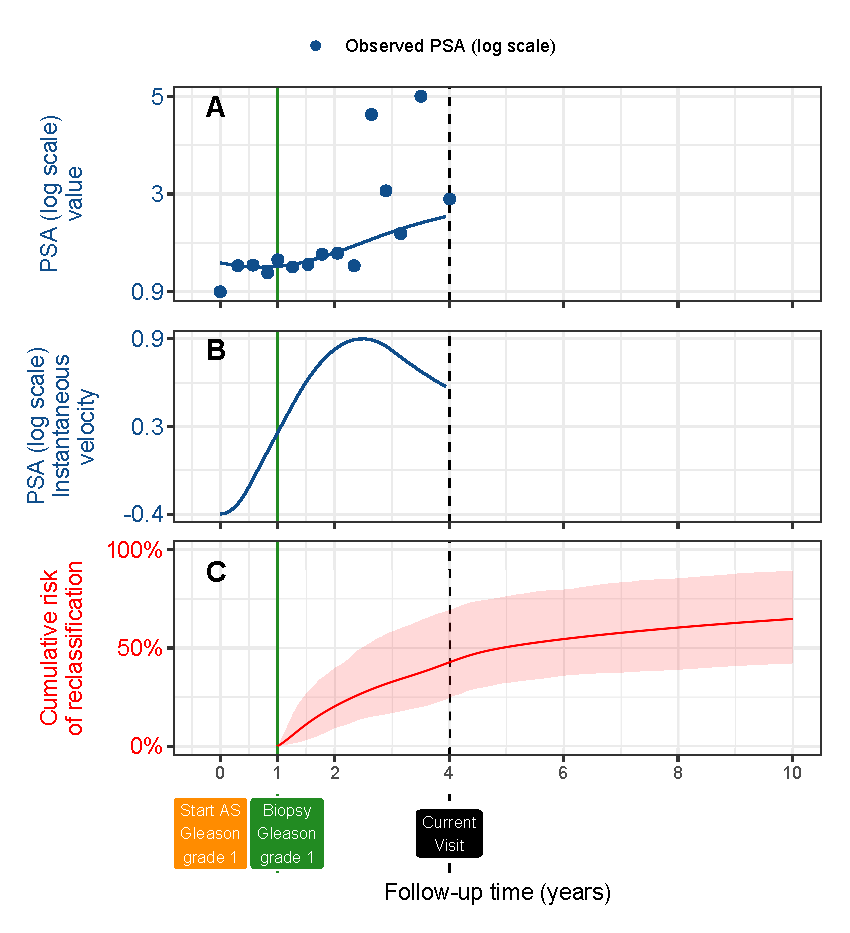
\includegraphics[width=\columnwidth]{images/jmExplanationPlot_113.eps}}
\caption{\textbf{Illustration of the joint model on a real PRIAS dataset patient}. \textbf{Panel~A:} Observed (blue dots) and fitted PSA (solid blue line) measurements, log-transformed. \textbf{Panel~B:} Estimated instantaneous velocity of PSA (log-transformed). \textbf{Panel~C}: Predicted cumulative-risk of reclassification (95\% credible interval shaded). Reclassification is defined as increase in Gleason grade \citep{epsteinGG2014} from grade~1 to 2 or higher. This risk of reclassification is available starting from the time of the latest negative biopsy (vertical green line at year 1 of follow-up). Joint model estimated it by combining the fitted PSA value and velocity (both on log scale of PSA) and time of latest negative biopsy. Black dashed line at year 4 denotes time of current visit.}
\label{fig:jmExplanationPlot_113}
\end{figure}

\subsection{Risk Predictions for Reclassification}
The key component in personalized schedules is the cumulative-risk of reclassification. For new patients, we predicted this risk over their whole follow-up period. To this end, we inputted their PSA measurements and Gleason grade results into the joint model fitted to the PRIAS dataset (e.g., Panel~C, Figure~\ref{fig:jmExplanationPlot_113}). When new PSA measurements or biopsy results become available over follow-up, the cumulative-risk profile is also updated.

We validated our prediction joint model using the PRIAS dataset (internal validation), as well using five largest AS cohorts from the GAP3 database \citep{gap3_2018} (external validation). These were University of Toronto AS (Toronto), Johns Hopkins AS (JHAS), Memorial Sloan Kettering Cancer Center AS (MSKCC), King's College London AS (KCL), and Michigan Urological Surgery Improvement Collaborative AS (MUSIC). We calculated the area under the receiver operating characteristic curve or AUC \cite{rizopoulos2017dynamic} as a measure of discrimination, and root mean squared prediction error or RMSPE \cite{rizopoulos2017dynamic} as a measure of calibration. Since AS studies are longitudinal in nature, we computed AUC and RMSPE in a time-dependent manner, at a gap of every six months (follow-up schedule of PRIAS) until year five (95-percentile of the observed reclassification times in PRIAS) of follow-up.

\subsection{Personalized Schedule of Biopsies, and Their Consequences}
Patients in PRIAS already have a follow-up schedule for testing PSA (Section~\ref{subsec:cohort}). We reused this schedule to create personalized biopsy schedules out of it. Specifically, we scheduled biopsy on a PSA visit if the predicted cumulative-risk of reclassification on that visit was more than 10\% (example threshold). We applied this rule of biopsy iteratively, starting from the current visit of a patient. After scheduling each subsequent biopsy, we updated the cumulative-risk of reclassification. This was done to account for the probability of not observing reclassification on the latest biopsy. We also kept a minimum gap of one year between consecutive biopsies (PRIAS recommendation). Personalized schedule using various risk thresholds are shown for an example patient in Figure~\ref{fig:demo_pat1}.

The choice of the risk threshold in the personalized schedule dictates the \textit{consequences} of that schedule. \textit{Consequences} are, the timing and total number of biopsies, and the expected delay in detecting reclassification if that schedule is followed. A larger risk threshold will lead to infrequent biopsies. However, it may also lead to a longer delay in detecting reclassification. To assist patients in choosing an appropriate risk threshold for personalized schedule, and to compare personalized and fixed schedules, we provided an estimate of these \textit{consequences}. These \textit{consequences} were also personalized (Appendix~C). That is, two patients may follow the same schedule of biopsies, but their expected delay in detection of reclassification will be different.

\subsection{Web-Application}
We implemented our methodology in a web-application \url{https://emcbiostatistics.shinyapps.io/prias_biopsy_recommender/}. This web-application uses the joint model that is fitted to the PRIAS dataset. Consequently, predictions for risk of reclassification can only be made for ten years of follow-up (follow-up period of PRIAS). Patient data can be uploaded in Microsoft Excel format, or entered manually on the web-application. Patients can check the evolution of their cumulative-risk of reclassification over the future follow-up visits. In addition, the web-application allows comparison of the following schedules: personalized schedules based on 5\%, 10\%, and 15\% risk threshold, annual and biennial biopsies, and the PRIAS schedule.

\begin{figure}[!htb]
\centerline{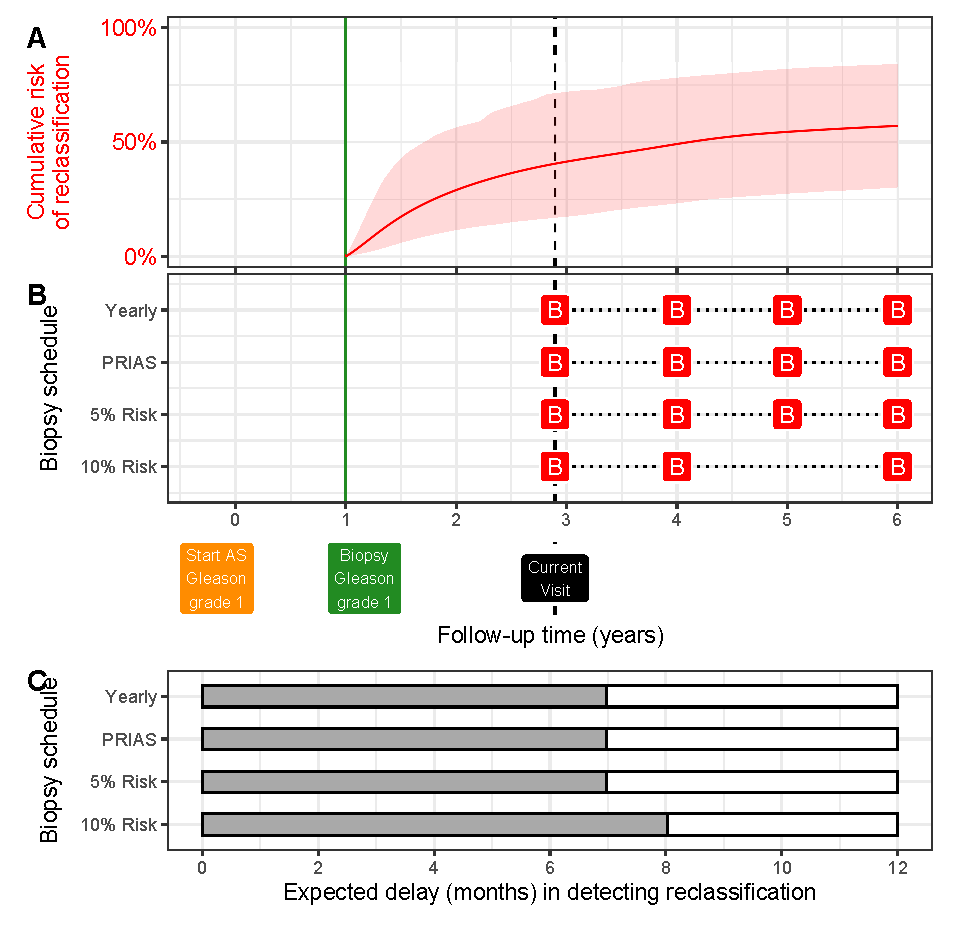
\includegraphics[width=\columnwidth]{images/demo_pat1.eps}}
\caption{\textbf{Illustration of personalized and fixed schedules of biopsies}. The PSA profile of this patient is shown in Figure~\ref{fig:jmExplanationPlot_113}. \textbf{Panel~A:} Predicted cumulative-risk of reclassification (95\% credible interval shaded). \textbf{Panel~B:} Personalized and fixed schedules of biopsies, with a red `B' indicating a scheduled biopsy. \textbf{Panel~C:}\ Expected delay in detecting reclassification for different schedules. Green vertical line at year 1 denotes time of latest negative biopsy. Black dashed line at year 4 denotes time of current visit.}
\label{fig:demo_pat1}
\end{figure}